\documentclass[11pt]{article}
\usepackage[T1]{fontenc}
\usepackage{lmodern,amsmath,amssymb,amsthm,mathtools,microtype,graphicx}
\usepackage[a4paper,margin=23mm]{geometry}
\usepackage[hidelinks]{hyperref}
\newtheorem{theorem}{Theorem}
\newtheorem{lemma}[theorem]{Lemma}
\title{Which original divisor words survive an Erd\H{o}s--Straus trace descent?}
\author{The Clankers}
\date{21 September 2026}
\begin{document}
\begin{center}
{\Large\bfseries Which original divisor words survive an\\
Erd\H{o}s--Straus trace descent?}\par\vspace{7pt}
The Clankers\quad---\quad21 September 2026
\end{center}
\begin{abstract}
For positive rational ES tails with integral sum, we determine exactly when
replacing the residual by a divisor preserves the original integer word and
produces an integral solution. Such a descent is guaranteed for all inputs
precisely for the nine words dividing 36. For each other word we construct
infinitely many hard-prime inputs for which every such return, including the
middle complement, fails. The primes still have explicit endpoint solutions.
Initial source occupancy at an arbitrary prime is not asserted.
\end{abstract}

Here ``hard prime'' means
$p\bmod840\in\{1,121,169,289,361,529\}$.

Let $p\equiv1\pmod4$ be prime, $p/4<a<p/2$ an integer, $R=4a-p$, and
$u\mid a^2$. Retain the E/M channel label and put
\[
 G_E=4u+1,\qquad G_M=p+4u,\qquad
 K(n)=\prod_{l^e\parallel n}l^{\lceil e/2\rceil},\qquad m=4K(u).
\]
The positive rational triples
\[
 E:\left(a,\frac{pa+a^2/u}{R},\frac{pa+p^2u}{R}\right),\qquad
 M:\left(a,\frac{p(a+a^2/u)}{R},\frac{p(a+u)}{R}\right)
\]
satisfy ES. Their tail sum is an integer exactly when $R\mid G_c^2$;
the common reduced denominator is $d=R/\gcd(R,G_c)$ and $d^2\mid R$.
Indeed their sums are $(a+pu)^2/(Ru)$ and $p(a+u)^2/(Ru)$, respectively.
We consider proper trace sources, where $d>1$. The word $u$ is an available
integer divisor, but the full residual gate is not yet satisfied.
These are the classical Type-I/II coordinates before the full gate, not an
alternative definition of ES \cite[Propositions 2.2 and 2.6]{ET}.

\begin{theorem}[The complete original return]
Every same-channel return keeping $p,u$ and replacing $R$ by a divisor is
indexed by exactly
\[
 \boxed{k\in\mathbb Z_{>0},\qquad k\mid R,\qquad d\mid k,
 \qquad k\equiv1\pmod{4K(u)}.}
\]
It gives $R'=R/k$, $a'=(p+R')/4$, $u'=u$ and $a'<a$.
\end{theorem}
\begin{proof}
The full target gate $R/k\mid G_c$ is equivalent to $d\mid k$.
The target integer denominator and word budget together are
$p+R/k\equiv0\pmod{4K(u)}$. The input gives $p+R\equiv0$ modulo the same
modulus, and $p$ is a unit there. Multiplication by $k$ proves the asserted
congruence equivalence. It also gives $k\equiv1\pmod4$, hence
$R'\equiv3\pmod4$, $3\le R'<R<p$ and the first-half range.

For a literal channel-labelled output put $g=\gcd(a',u)$,
$(h,r,s)=(g^2/u,u/g,a'/g)$. Prime valuations give positive integers with
$a'=hrs$, $u=hr^2$, $\gcd(r,s)=1$. For E use
$\kappa=(pr+s)/R'$ and $(a',hs\kappa,phr\kappa)$; for M use
$\lambda=(r+s)/R'$ and $(a',phs\lambda,phr\lambda)$.
The gates prove integrality, and multiplication verifies the identity.
The respective labelled inverses are $a'^2/(R'y-pa')$ and
$pa'^2/(R'y-pa')$.
\end{proof}

Here and below $k$ is a positive integer.  The full inverse fibre above a fixed
original target satisfying $R'=4a'-p$, $3\le R'<p$, $R'\equiv3\pmod4$,
$u\mid(a')^2$, and $R'\mid G_c$ retains all
$1\le k\le(p-1)/R'$ with $k\equiv1\pmod{4K(u)}$,
$R'k\mid G_c^2$, and $R'k\nmid G_c$. Set $R=R'k$ and $a=(p+R)/4$.
Thus coefficient aggregation is over known finite fibres, not over unmarked
residue support.

Write $R=\delta t^2$ with $\delta$ its squarefree part, and $q_0=K(d)$.
Then $q_0\mid t$. The square deletions are exactly
\[
 k=q^2,\qquad q_0\mid q\mid t,\qquad q^2\equiv1\pmod{4K(u)}.
\]

\begin{theorem}[Exact universal seed list]
For a fixed positive integer $u$, every proper trace source at every prime
$p\equiv1\pmod4$ has the preceding return if and only if
\[
 \boxed{u\in\{1,2,3,4,6,9,12,18,36\}.}
\]
For each listed word, $q=q_0$ gives a one-step return. Its complete square-deletion
family has $\tau(t/q_0)$ distinct original targets.
\end{theorem}
\begin{proof}
A modulus $m$ divisible by four has every unit square equal to one exactly when
$m\mid24$. To check this directly, an odd prime power has exactly two solutions
to $x^2=1$; modulus four has two and $2^\alpha$, $\alpha\ge3$, has four.
Counting the kernel of the square map proves that its image has order
\[
 2^{\max(0,\alpha-3)}
 \prod_{i=1}^{r}l_i^{e_i-1}(l_i-1)/2,
\]
for $m=2^\alpha\prod_{i=1}^{r}l_i^{e_i}$ with distinct odd $l_i$.
It is one precisely for $m=4,8,12,24$, equivalently $K(u)\mid6$ or $u\mid36$.
All available $q$ are units modulo $m$. Thus for these words every $q_0\mid q\mid t$
works, giving the stated count and strict descent.

For necessity let $m=4K(u)\nmid24$. Choose a unit $b\bmod m$ with $b^2\ne1$;
replace its sign to arrange $b\equiv1\pmod4$.
Dirichlet's theorem \cite[Theorem 18.1]{Dirichlet} gives distinct primes
\[
 \delta\equiv-b^2\pmod m,\qquad t\equiv b^{-1}\pmod m,
 \qquad \delta,t>\max(u,7).
\]
Thus $\delta\equiv3\pmod4$, $t\equiv1\pmod4$ and both are coprime to
$L=\operatorname{lcm}(840,m)$. Set $R=\delta t^2$, and take a prime
$e\equiv3\pmod4$ coprime to $LR$. The reduced CRT class
\[
 p\equiv1\pmod L,\qquad p\equiv\delta t-4u\pmod R,
 \qquad p\equiv-1\pmod e
\]
contains infinitely many primes. Take $p>\max(R,e,B(u)R)$, where
$B(u)=\prod_l l^{\lfloor v_l(u)/2\rfloor}$.
Since $840\mid L$, all these primes lie in the hard class $1\pmod{840}$.
Then $a=(p+R)/4$ is an integer multiple of $K(u)$, since $R\equiv-1\pmod m$.
The original M word $u\mid a^2$ has exact denominator $d=t>1$.

The only candidate target residuals dividing $R$, dividing $p+4u$, and
congruent to three modulo four are
$\delta,\delta t,R$. The last fails the gate. The first two fail the word budget:
$p+\delta\equiv1-b^2\ne0$ and $p+\delta t\equiv1-b\ne0$ modulo $m$.
Even the other middle orientation cannot escape: for $u^*=a^2/u$,
$4K(u^*)=(p+R)/B(u)>R$.  Moreover
$4u(p+4u^*)\equiv p(p+4u)\pmod R$, so its exact denominator remains
$t>1$.  Thus no allowed deletion factor can be one modulo its budget.

These are not ES counterexamples. Put $c=(p+1)/e$ and $j=(e+1)/4$.
The original middle state $(h,r,s,\lambda)=(j,1,c,1)$ returns
$(jc,pjc,pj)$. Its first-half range follows from $c(e-1)>2$.
This supplies a genuine solution at every prime used in the obstruction.
\end{proof}

\paragraph{Why full multiplicities and non-square deletions matter.}
At $p=1009,a=321,R=275,u=9$, the proper M trace has tails
$215926/5,6054/5$. The old full E and M gates are both empty, but $k=25$ returns
\[
 \frac4{1009}=\frac1{255}+\frac1{686120}+\frac1{24216}.
\]
At $p=51361,a=14845,R=8019,u=5$, the sole deletion is $k=81$ and the new
residual is $99$, still containing a square. Stripping every square instead
loses the original word. At $p=1108801,a=279295,R=8379,u=5$, the complete deletion
set is $\{21,441\}$: an additional available factor seven repairs the residue
of the forced factor three. Its integer coefficient is two, not an absent
coefficient after reduction modulo two; the two labelled representatives are
$v=7,147$, while the retained original word is the single word $u=5$.

The complete proof and executable certificates retain the inverse fibres and
original coefficient counts. A trace source is not guaranteed at every prime;
universal ES occupancy and historical priority are not claimed.

\begin{figure}[htbp]
\centering
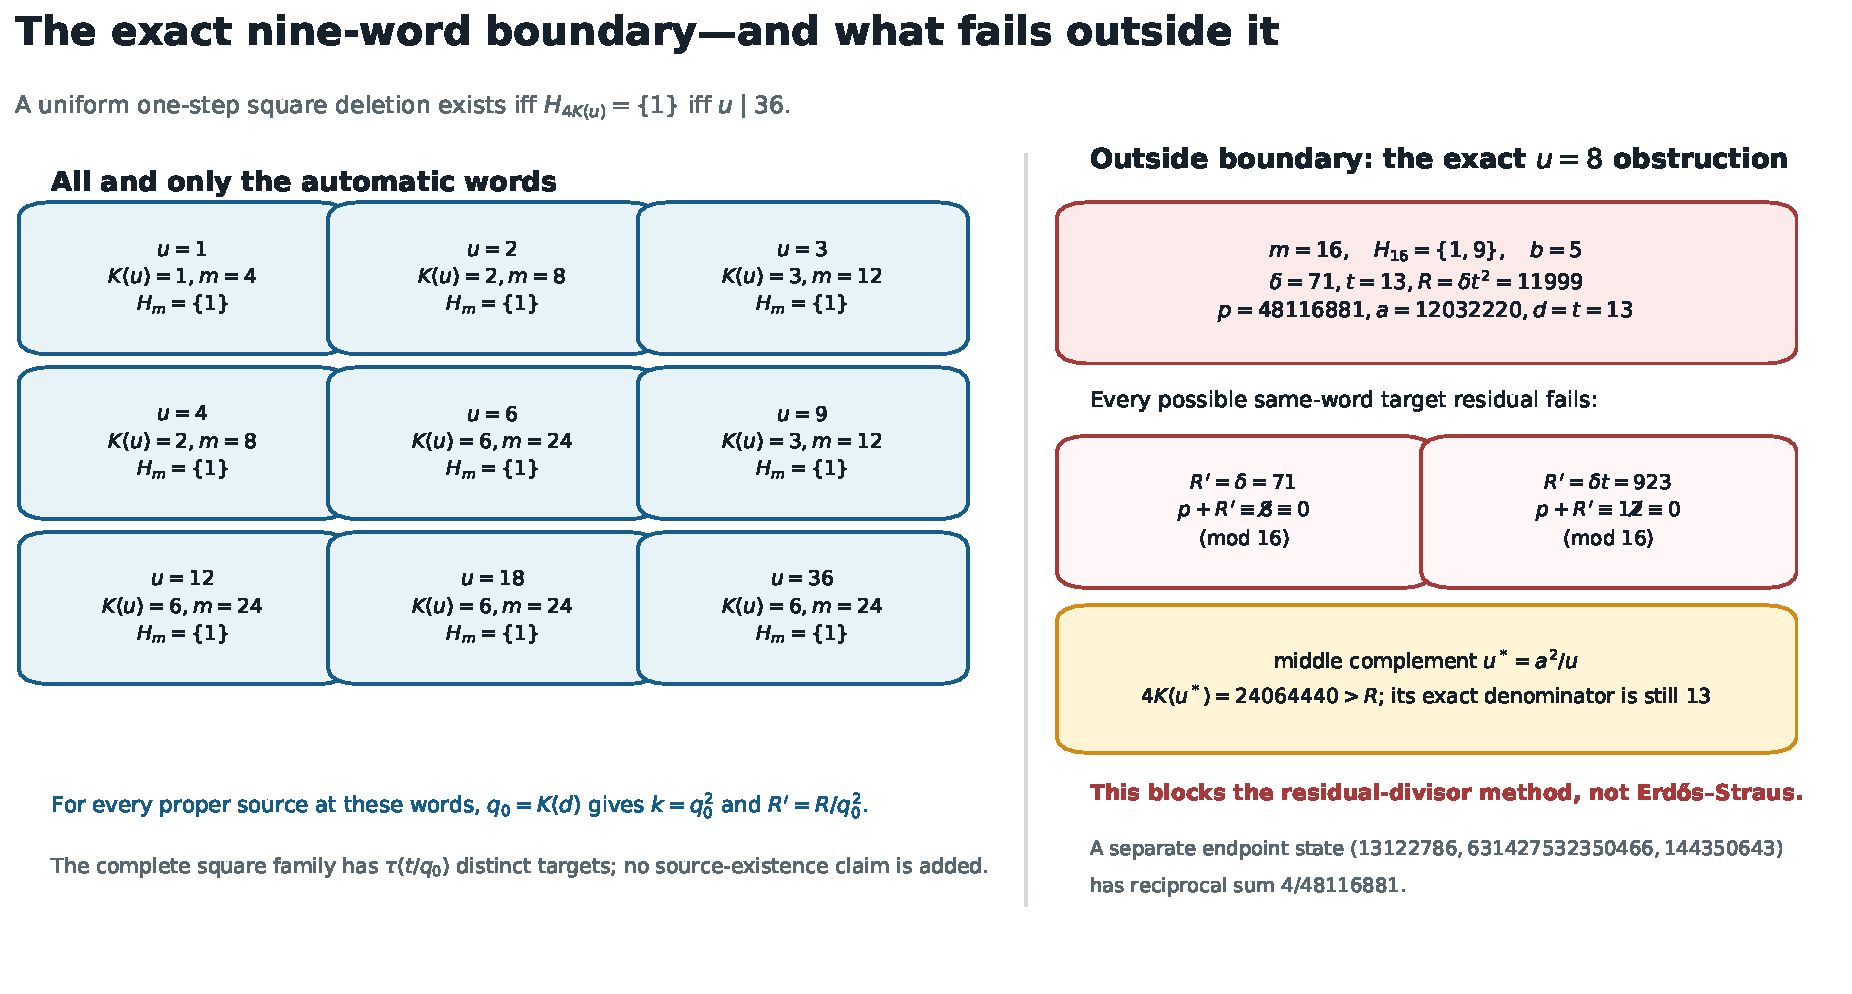
\includegraphics[width=\textwidth]{figures/nine_word_boundary.pdf}
\caption{The exact universal nine-word boundary and the explicit $u=8$
obstruction to the residual-divisor method.  The obstruction prime has a
separately displayed integer ES endpoint and is not an ES counterexample.}
\end{figure}

{\small
\begin{thebibliography}{2}
\setlength{\itemsep}{0pt}
\bibitem{ET} Elsholtz, C., \& Tao, T. (2013). Counting the number of solutions to
 the Erd\H{o}s--Straus equation on unit fractions. \emph{J. Austral. Math. Soc., 94},
 50--105. arXiv:1107.1010, \S2,
 \href{https://arxiv.org/pdf/1107.1010\#page=12}{Proposition 2.2} and
 \href{https://arxiv.org/pdf/1107.1010\#page=14}{Proposition 2.6}.
\bibitem{Dirichlet} Sutherland, A. V. (2017). \emph{18.785 Lecture 18:
 Dirichlet $L$-functions, primes in arithmetic progressions}. MIT,
 \href{https://math.mit.edu/classes/18.785/2017fa/LectureNotes18.pdf\#page=1}{Theorem 18.1}.
\end{thebibliography}
}
\end{document}
